
\section{Background}\label{sec:background}

Some basic concepts of solid modeling, and in particular the foundational idea of representation scheme, as well as few basic concepts of algebraic topology, are shortly introduced in this section, including the computation of the matrix of a boundary operator between chain spaces.

\subsection{Representation Schemes}\label{sec:schemes}

A \emph{representation scheme} for solid modeling is a mapping between a space of mathematical models and  space of symbolic representations like generated by a formal grammar.
Solid pointsets (i.e., `$r$-sets') are defined~\cite{Requicha:1980:RRS:356827.356833} as compact (bounded and closed) regular and semianalytic subsets of the $d$-space. A large number of representation schemes were defined in the past forty years, including the two main classes of (a) \emph{boundary representations} (`$B$-reps'), where the solid model is represented through a representation of its boundary elements, i.e.~faces, edges and vertices, and (b) \emph{decompositive/enumerative representations}, that are a decomposition of either the object or the embedding space, respectively, into a well-defined \emph{cellular complex}. In particular, a boundary representation provides a cellular decomposition of the object's boundary into \emph{cells} of dimension zero (vertices), one (edges), and two (faces). Medical imaging can be classified as the \emph{enumerative representation} of cellular decompositions of organs and tissues of interest, in particular, as subsets \emph{of 3D volume elements} (voxels) from the 3D image. 


\subsection{Linear Algebraic Representation}\label{sec:lar}


The \emph{Linear Algebraic Representation} (\textsc{lar}), introduced in~\cite{Dicarlo:2014:TNL:2543138.2543294}, aims to represent the \emph{chain complex}~\cite{TSAS} generated by a piecewise-linear \emph{geometric complex} embedded either in 2D or in 3D. In a few words, it gets a minimal characterization of geometry and topology of a cellular complex, i.e.~the embedding mapping $\mu : C_0 \to \E^d$ of 0-cells (vertices), as well a description of $(d-1)$-cells as subsets of vertices, and is able to return the whole chain complex 
\begin{equation}
C_\bullet = (C_p, \partial_p) := 
C_3 
\substack{
\delta_2 \\
\longleftarrow \\
\longrightarrow \\
\partial_3 
}
C_2 
\substack{
\delta_1 \\
\longleftarrow \\
\longrightarrow \\
\partial_2 
}
C_1  
\substack{
\delta_0 \\
\longleftarrow  \\
\longrightarrow \\
\partial_1 
}
C_0 .
\end{equation}



%\[ 
%C_\bullet = (C_p, \partial_p) := 
%C_3 \ 
%\substack{
%\delta_2 \x
%\longleftarrow \[-1mm]
%\longrightarrow \
%\partial_3 
%}
%\ C_2 \ 
%\substack{
%\delta_1 \
%\longleftarrow \[-1mm]
%\longrightarrow \
%\partial_2 
%}
%\ C_1 \ 
%\substack{
%\delta_0 \
%\longleftarrow \[-1mm]
%\longrightarrow \
%\partial_1 
%}
%\ C_0 .
%\] 

% {   
%   \centering\vspace{1mm}
%   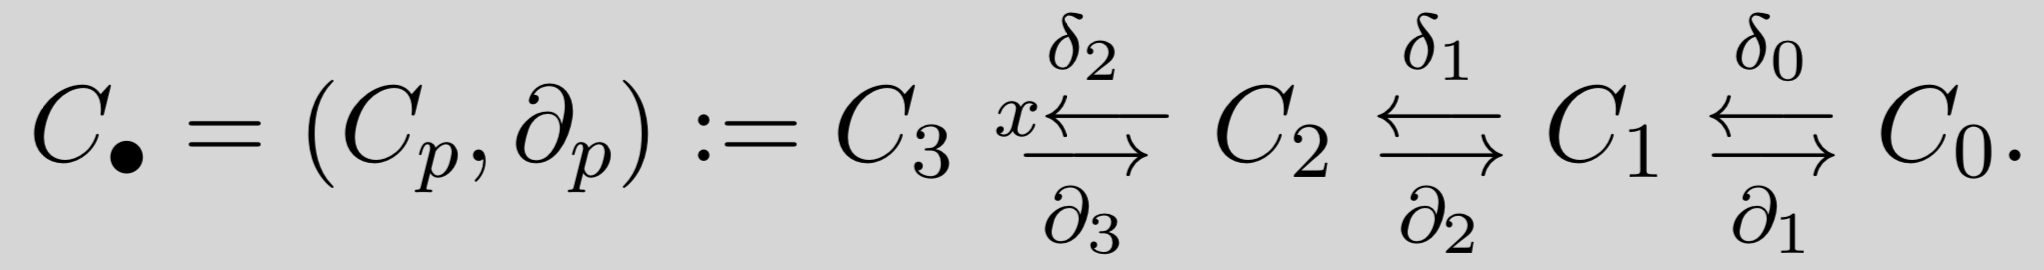
\includegraphics[width=0.475\textwidth]{figs/complex} 

% }

\noindent
and, in particular, any basis for linear chain spaces $C_p$, and any linear
boundary/coboundary map \(\partial_p\) and
\(\delta_p=\partial_{p-1}^\top\) between them. The \emph{domain} of \textsc{lar} is the set of \textbf{chain complexes} generated by cell $d$-complexes ($2\leq d\leq 3$). The computer \emph{representations} of \textsc{lar} are \textbf{sparse binary matrices} to represent both the operators and the chain bases. Note that in algebraic topology a $p$-chain is defined as a linear combination of $p$-cells with scalars from a field. When the scalar coefficients are from $\{-1, 0, +1\}$, a chain may represent \emph{any (oriented) subset of cells} from the cellular complex.
Scalars from $\{0, 1\}$ are used for non-oriented complexes.

We may, therefore, get the $(p-1)$-boundary $\partial_p c_p$ of \emph{any} $p$-chain $c_p$, by multiplication of the coordinate representation $[\partial_p]$ of the boundary operator times the coordinate representation $[c_p]$ of the chain in terms of such scalars, i.e.~by a  matrix-vector product $ [\partial_p] [c_p] $.

It is possible to show that the \textsc{lar} representation scheme is very expressive, i.e.~that it  has a large domain,  including collections of: line segments, quads, triangles, polygons, meshes;  pixels, voxels, volume images; B-reps, enumerative and decompositive representations of solids. 
In this paper we apply \textsc{lar} methods to computation of boundary representations of solid models from segmentation (labeling) of 3D medical images.
To display a triangulation of  boundary faces  in their proper position in space, the information required is contained in the \emph{geometric chain complex} (GCC):
\[
\mu: C_0\to\E^3,\ (\delta_0, \delta_1, \delta_2)
\qquad\equiv\qquad
\texttt{(geom, top) = (V, (EV, FE, CF))}
\]
The GCC allows to transform the (possibly non connected) boundary 2-cycle of surfaces as a standard B-rep~\cite{shapiroSM:202}. 
The geometry \texttt{geom} is given by
the embedding matrix \texttt{V} of vertices (0-cells), and  topology \texttt{top} by the three sparse matrices (\texttt{EV}, \texttt{FE}, \texttt{CF}) of coboundaries ($\delta_0, \delta_1, \delta_2$) of the chain complex describing a   
space arrangement~\cite{paoluzzi2019finite}.
Note that ordered pairs of letters from \texttt{V,E,F,C}, correspond to \emph{\emph{\texttt{V}}ertices$\to$\emph{\texttt{E}}dges$\to$\emph{\texttt{F}}aces$\to$\emph{\texttt{C}}ells} into the 
\emph{\emph{\texttt{C}}olumn$\to$\emph{\texttt{R}}ow} order of matrix maps of operators.



\subsubsection*{Construction of boundary matrix $\partial_d$}

First, let us fix an ordering for all the cells of a partition of input data (with vertices $V$, edges $E$, pixels $F$, and voxels $C$), i.e.~for each 0-, 1-, 2-, and 3-elements of a cell partition \texttt{V,E,F,C} of a 3D image, i.e., once fixed the $p$-bases for linear spaces $C_p$ of $p$-chains $(0\leq p\leq 3)$, we call $M_p = (m_{i,j})$ the \emph{characteristic matrix} of the $p$-basis, expressed as subsets so that 
$m_{i,j}=1$ if and only if the $j$-th  $0$-cell $c^j_0$ belongs 
% , where  we have that $m_{i,j}=1$ if and only if the $j$-th $0$-cell belongs 
to the boundary of $i$-th $p$-cell $m_{i,j}$, and $m_{i,j}=0$ otherwise.  

Let us note that the product of binary matrices is not binary, so by computing the (sparse) matrix product $(M_{p-1} M_{p}^t) = (n_{i,j})$, with $n_{i,j} = \sum_{k} m_{i,k}m_{k,j}$, we get for each $n_{ij}$ the \emph{number of vertices} shared by $c_{p-1}^i$ and $c_{p}^j$. When this number equates the cardinality of $c_{p-1}^i$, this elementary chain is contained on the boundary of $c_{p}^j$. In a volumetric data, with cubic 3-cells and squared 2-cells in-between, everywhere we get $n_{i,j}=4$, we may state $c_{2}^i\subset\partial c_{3}^j$. Therefore, in each $j$ column of $M_{2} M_{3}^t = (n_{i,j})$, we have exactly \emph{six rows} where  $n_{i,j} = 4$, since a cube (3-chain) has six boundary faces (2-chains). The unit incidence coefficients in $\left[\partial_3\right]$ are accordingly located by filtering the coefficients with value 4.

Finally, consider the linear graded boundary operator $\partial_p : C_p \to C_{p-1}$. As such, it contains by columns the representation of domain basis elements, expressed as a linear combination of the basis elements of the range space. Therefore, the operator matrix $[\partial_d]$ is readily obtained by setting $[\partial_d](i,j)=1$ if $n_{i,j}=4$ and $[\partial_d](i,j)=0$ otherwise.  Of course, it will contain six non-zero elements for the column.  It may be worth remembering every 3-cell (voxel) of the volumetric data has exactly six 2-faces. 

It is possible to show that all the interesting relations of incidence/adjacency between cells of different dimensions can be both computed and efficiently queried by pairwise computing some matrix products, with one of terms possibly transposed, using only the two boundary and coboundary operator matrices $[\partial_p]$ and $[\delta_p]$, and where $[\delta_p] = [\partial_p^\top]$. We~may also show that such matrices are \emph{very sparse}, with their sparseness growing rapidly with the dimensions (see Section~\ref{sec:block}). The pattern of non-zeros in matrix $[\partial_3]$ corresponding to a brick of shape $(4,4,4)$ is given in Fig.~\ref{fig:boundary_matrix_4x4x4}.

\begin{figure}[tbp] %  figure placement: here, top, bottom, or page
   \centering
   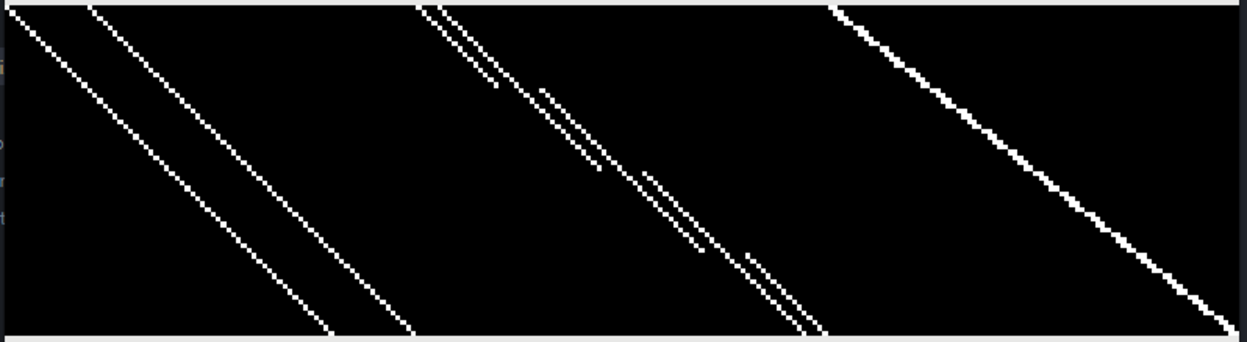
\includegraphics[width=0.75\linewidth]{figs/boundary_matrix_4x4x4.pdf} 
   \caption{
   The binary image of \emph{sparse} coboundary matrix  $\left[\delta_2\right] = \left[\partial_3\right]^t : C_2 \to C_3$,
%   The binary image of the coboundary operator  $\delta_2 = \partial_3^\top : C_2 \to C_3$, 
   built for a small volumetric data (or a brick) with shape $(4,4,4)$. Note that the number of rows equates the size $4\times 4\times 4 = 64$ of the voxel set; the number of columns is $d\,n\,(1+n)^{d-1} = 3\times 4\times 25 = 300$. Of course, the number of non-zeros per row (cardinality of the facet set of a single voxel) is six, whereas the number of non-zeros per column is two, but on boundary facets.}
   \label{fig:boundary_matrix_4x4x4}
\end{figure}

\subsection{Multiindices from Cartesian indices}\label{sec:inds-from-cart}

In order to utilize the topological algebra shortly recalled in this paper, we need to explicitly sort the cells of the various dimensions into linearly ordered sequences, possibly according to the linear order their information is linearly accommodated in computer storage. 

\subsection{Taubin Smoothing}\label{sec:taubin}

Every boundary chain extracted from an image block $\B(i,j,k,n)$ is a \emph{2-cycle}, i.e., a closed 2-chain---in other words, a 2-chain with empty boundary. Such 2-cycles are joined together by removing the double 2-cells (at the boundaries of adjacent bricks) after having suitably shifted their indices to an unique linear representation of the whole image. The resulting raster surface is made by mutually orthogonal raster facets, that must be smoothed in order to get a fair surface. A linear time and space algorithm for this purpose is the Laplacian smoothing, which iteratively  moves each vertex (0-cell) to the centroid of its neighbors. A well known weakness of this simple algorithm is the asymptotic convergence of the whole mesh to a single point, resulting in unfair size reduction even after few iterations.  Conversely, the Taubin smoothing algorithm~\cite{Taubin:1995:SPA:218380.218473,egst.20001029} alternates two Laplacian smoothing steps with \emph{shrink} and \emph{inflate} effects respectively, with the result of delivering pretty invariant sizes and volume of the smoothed mesh. The best results are obtained on meshes which have small variations of edge length and face angles, like for surfaces extracted from 3D raster images, as in our case.
 

